\chapter{Estado del Arte}\label{ch:Estado del Arte}
Para la correcta comprensión del trabajo presente, se necesita conocer el estado actual de las herramientas y tecnologías disponibles para el cálculo y la visualización de series de Fourier, así como los estudios y proyectos previos que abordan la implementación de soluciones similares. En este sentido, se revisarán diversas plataformas de uso común que permiten realizar estos procesos de manera separada, además de destacar trabajos académicos relacionados que aportan al desarrollo de herramientas educativas y matemáticas interactivas. Esta revisión permitirá contextualizar la propuesta de una aplicación web que integre ambas funcionalidades en una sola plataforma.

\section{Herramientas y Tecnologías Actuales}
En esta sección se presentarán las principales herramientas tecnológicas utilizadas para el cálculo de series de Fourier y su visualización gráfica. Podemos verlos en la siguiente tabla:

\begin{longtable}{ | m{2.5cm} | m{6.5cm} | m{4cm} | }
	\rowcolor{black!75}
	\head {SOFTWARE} & \head {CARACTERÍSTICAS} & \head {PRECIO} \\ \hline
	\endfirsthead
	\multicolumn{3}{c}{{\tablename\ \thetable{} -- continuación}} \\
	\rowcolor{black!75}
	\head {SOFTWARE} & \head {CARACTERÍSTICAS} & \head {PRECIO} \\ \hline
	\endhead
	\hline \multicolumn{3}{r}{{Continúa en la siguiente página}} \\
	\endfoot
	\hline
	\endlastfoot
	Wolfram Alpha & Se trata de un potente motor comercial de conocimiento computacional para cálculos matemáticos y gráficos. Contiene módulos que permiten el calculo de los coeficientes de Series de Fourier (Trigonométrica y compleja) así como las extensiones pares e impares para funciones simples o a trozos, así como poder expandir la serie y obtener una gráfica estática.~\cite{wolfram2024}  & Desde MXN \$1,200.00 anuales para estudiantes, plan gratuito limitado. \\ \hline
	Geogebra & Herramienta dinámica para construcciones geométricas y gráficas. Podemos graficar cualquier serie o extensión trigonométrica y poder ver como cambia la serie conforme añadimos más coeficientes. Requiere que hagamos los cálculos y armar la expresión de la serie~\cite{GeoGebra2024} & Software libre y código abierto \\ \hline
	Desmos  & Similar a Geogebra es una calculadora gráfica en línea para cálculos y gráficos, donde de igual modo podemos graficar cualquier serie o extensión trigonométrica y poder ver como cambia la serie conforme añadimos más coeficientes. Requiere cálculos previos para series de Fourier.~\cite{Desmos2024} & Software libre y código abierto\\ \hline
	Python$_{Manim}$ & Librería de animación en Python para visualizaciones matemáticas, incluida la animación de series de Fourier. Podemos graficar cualquier serie ya sea trigonométrica o exponencial y poder animar de infinitas maneras el como se aproxima la serie con sus coeficientes. Requiere hacer los cálculos, armar la expresión de la serie y tener conocimientos en Python, programación orientada a objetos y a librería de Manim ~\cite{Manim2024} & Software libre y código abierto \\ \hline
	Python$_{SymPy}$ &Es una biblioteca de Python para realizar matemáticas simbólicas, que incluye el cálculo de series de Fourier. A menudo se usa en combinación con librerías de visualización como Matplotlib para representar gráficamente los resultados, pero de nuevo, esta combinación requiere conocimientos de programación.~\cite{Matplotlib-sympy2024} & Software libre y código abierto \\ \hline
	Matlab  & Es un entorno de programación comercial para cálculos numéricos y visualización de datos, con herramientas específicas para series de Fourier, además de tener funciones para poder graficarlas. Requiere conocimientos en matlab.~\cite{MathWorks2024} & Desde USD\$99 (aprox. MXN\$1627.82) anuales para estudiantes.\\ \hline	
	\rowcolor{white}\caption{Comparación de software para cálculos matemáticos y visualización de datos} \label{tabla:software} \\
\end{longtable}


\subsection{Comparativa del Funcionamiento de las Herramientas}

A continuación, se procederá a calcular la serie de Fourier para la función \( f(x) = x \) en el intervalo de \(-\pi\) a \(\pi\) utilizando cada una de las herramientas previamente descritas. El cálculo se realizará en su \textbf{forma trigonométrica} y, en los casos en que la herramienta lo permita, también se obtendrá la \textbf{forma exponencial compleja}. Asimismo, se graficará la serie de Fourier en las plataformas que lo permitan, lo que nos permitirá comparar tanto el proceso como los resultados obtenidos en cada herramienta. \newline

Esta comparación servirá para identificar las capacidades, ventajas y limitaciones de cada una de las plataformas en el contexto del cálculo y la visualización de series de Fourier, evaluando también su facilidad de uso y precisión en la representación gráfica.\newline

Primeramente, calcularemos la serie nosotros para hacer una comparativa con los resultados dados por los softwares:\newline
Los coeficientes de Fourier para la función \( f(x) = x \), en el intervalo \( [-\pi, \pi] \), son los siguientes (ver \hyperref[app:Estado-del-arte-coeff]{Apendice A} para los cálculos completos):

- **Forma Trigonométrica**:
\[
a_0 = 0, \quad a_n = 0, \quad b_n = \frac{2 (-1)^{n+1}}{n}
\]

Por lo tanto, la serie trigonométrica de Fourier para \( f(x) = x \) es:

\[
f(x) = 2 \sum_{n=1}^{\infty} \frac{(-1)^{n+1}}{n} \sin(n x)
\]

- **Forma Exponencial Compleja**:
\[
c_n = \frac{i (-1)^n}{n}, \quad \text{para } n \neq 0.
\]

Por lo tanto, la serie exponencial compleja de Fourier para \( f(x) = x \) es:

\[
f(x) = \sum_{\substack{n=-\infty \\ n \neq 0}}^{\infty} \frac{i (-1)^n}{n} e^{i n x}
\]

\begin{figure}[h]
	\centering
	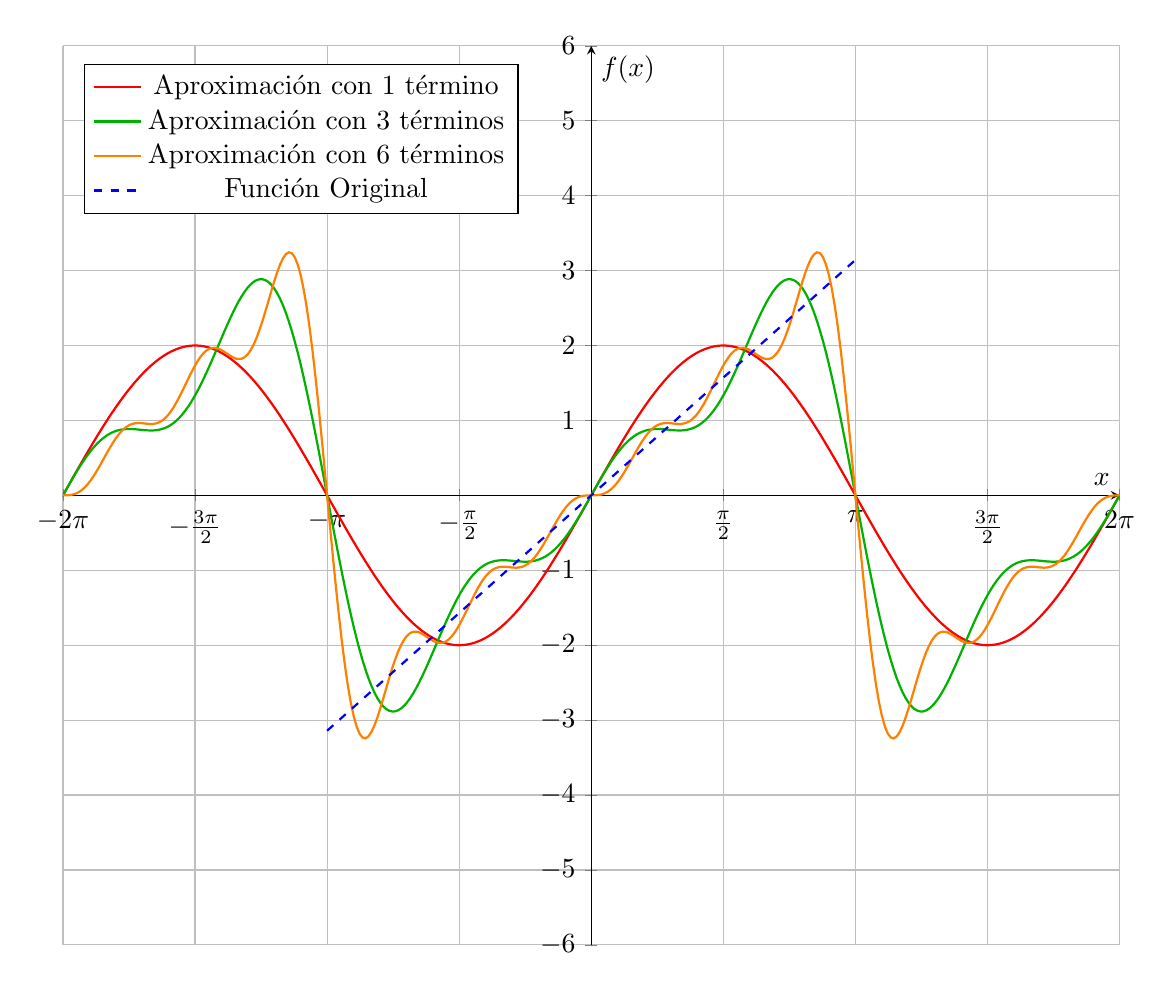
\begin{tikzpicture}
		\begin{axis}[
			axis lines=middle,
			grid=both,
			enlargelimits=false,
			width=15cm, % Ancho de la gráfica
			height=13cm, % Altura de la gráfica
			xlabel=$x$,
			ylabel={$f(x)$},
			xtick={-6.28319, -4.7123889, -3.14159, -1.5708, 0, 1.5708, 3.14159, 4.7123889, 6.28319},
			xticklabels={$-2\pi$, $-\frac{3\pi}{2}$, $-\pi$, $-\frac{\pi}{2}$, $0$, $\frac{\pi}{2}$, $\pi$, $\frac{3\pi}{2}$, $2\pi$},
			ymin=-6, ymax=6,
			xmin=-2*pi, xmax=2*pi,
			samples=400,
			domain=-7:7,
			legend style={at={(0.02,0.98)}, anchor=north west},% Posición ajustada a la esquina superior izquierda
			axis background/.style={fill=white}
			]
			
			% Aproximación con 1 término
			\addplot[red, thick] {2*( sin(180*x/pi)/1 )};
			\addlegendentry{Aproximación con 1 término};
			
			% Aproximación con 3 términos
			\addplot[green!70!black, thick] {2*( sin(180*x/pi)/1 - sin(180*2*x/pi)/2 + sin(180*3*x/pi)/3 )};
			\addlegendentry{Aproximación con 3 términos};
			
			% Aproximación con 6 términos
			\addplot[orange, thick] {2*( sin(180*x/pi)/1 - sin(180*2*x/pi)/2 + sin(180*3*x/pi)/3 - sin(180*4*x/pi)/4 + sin(180*5*x/pi)/5 - sin(180*6*x/pi)/6 )};
			\addlegendentry{Aproximación con 6 términos};
			
			% Función Original (línea punteada)
			\addplot[blue, thick, dashed, domain=-pi:pi] {x};
			\addlegendentry{Función Original};
			
		\end{axis}
	\end{tikzpicture}
	\caption{Gráfica de los coeficientes de Fourier calculados en el \hyperref[app:Estado-del-arte-coeff]{Apendice A}  \textit{Fuente: Elaboración propia}}
	
	\label{fig:fourier-estado-del-arte}  % Etiqueta para la figura
\end{figure}


Podemos ver en la \hyperref[fig:fourier-estado-del-arte]{Figura 2.1}, la gráfica de la función y sus aproximaciones de Fourier, donde estas aproximaciones son equivalentes entre la serie trigonométrica y la serie exponencial

\subsubsection{Cálculo de Serie de Fourier con Wolfram Alpha}
WolframAlpha nos permite calcular series de Fourier trigonométricas y exponenciales complejas, además de que nos permite calcular extensiones de medio rango periódicas pares, impares y periódicas.
Para nuestra primer prueba, calcularemos la serie de Fourier trigonométrica para la función \( f(x) = x \) en el intervalo de \(-\pi\) a \(\pi\), para hacerlo usaremos la función \emph{FourierTrigSeries(exp, t, n)} de WolframAlpha, que nos permite calcular la serie trigonométrica de Fourier de la función \emph{exp} respecto a la variable \emph{t} obteniendo la serie hasta el término \emph{n}.
\begin{figure}[H]
	\centering
	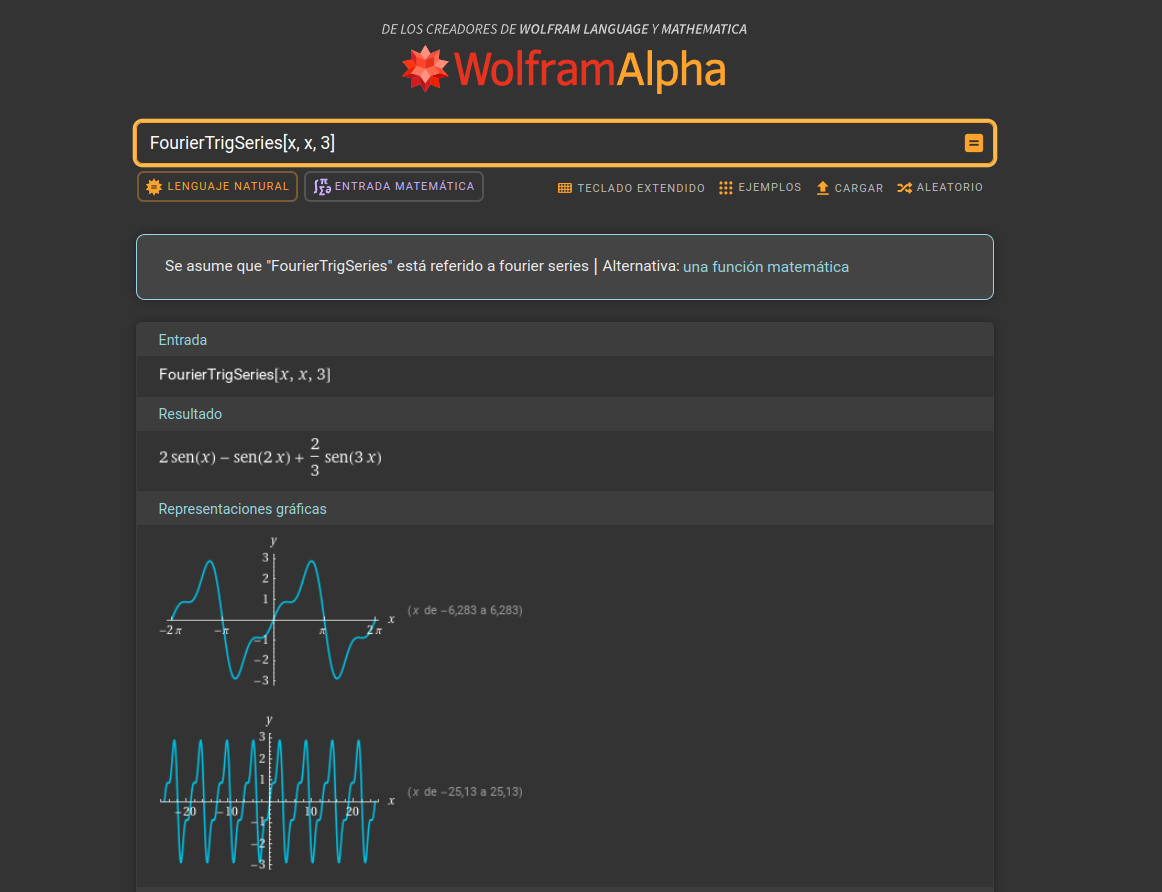
\includegraphics[width=0.9\textwidth]{img/chapter02/wolfram_trig_series.png}
	\caption{Calculo de una serie trigonométrica de Fourier en WolframAlpha}
	\label{fig:wolfram-trig-series}  % Etiqueta para la figura
\end{figure}
Ahora usaremos la función de \emph{FourierSeries(exp, t, n)} de WolframAlpha, esta función no permite calcular la serie exponencial compleja de Fourier de la función \emph{exp} respecto a la variable \emph{t} obteniendo la serie hasta el término \emph{n}.
\begin{figure}[H]
	\centering
	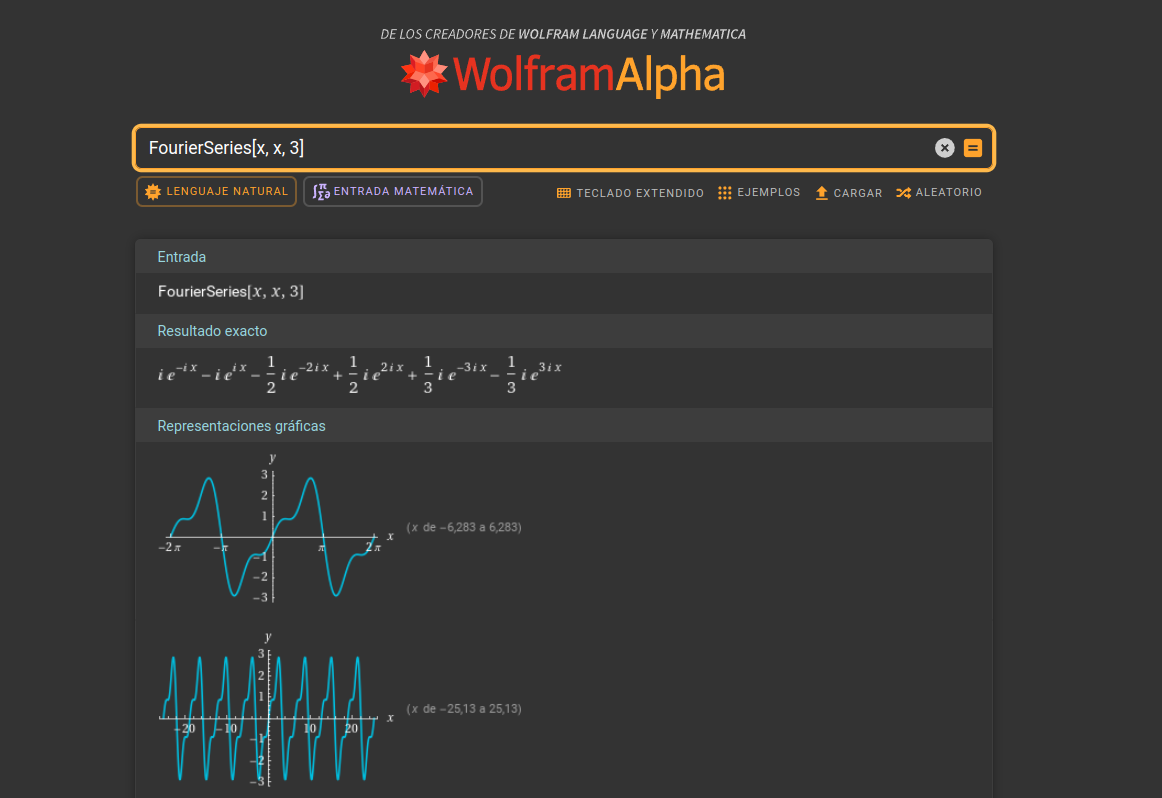
\includegraphics[width=0.9\textwidth]{img/chapter02/wolfram_complex_series.png}
	\caption{Calculo de una serie trigonométrica de Fourier en WolframAlpha}
	\label{fig:wolfram-exp-series}  % Etiqueta para la figura
\end{figure}
Wolfram nos devuelve la expansión de cada serie en su forma mas reducida, ademas de dos pequeñas gráficas de nuestra aproximación vista desde  no nos devuelve los coeficientes de la serie ni tampoco su expresión final en notación de serie.

\subsubsection{Cálculo de Serie de Fourier con MATLAB}
Matlab 

\subsubsection{Cálculo de Serie de Fourier con GeoGebra}

Aquí se describirá cómo se realiza el cálculo y la graficación de la serie de Fourier utilizando GeoGebra...

\subsubsection{Cálculo de Serie de Fourier con Python (Matplotlib/Manim)}

Aquí se describirá cómo se realiza el cálculo y la graficación de la serie de Fourier utilizando Python con las librerías Matplotlib o Manim...



\section{Trabajos y Proyectos Relacionados}
En esta sección se analizarán trabajos académicos y proyectos de investigación que han desarrollado herramientas similares o que abordan la enseñanza de series de Fourier y el uso de plataformas interactivas para la educación matemática. 

%\begin{table}[h]
%	\centering
%	\begin{tabular}{ | m{2.5cm} | m{6.5cm} | m{4cm} | }
%		\rowcolor{black!75}
%		\head {SOFTWARE} & \head {CARACTERÍSTICAS} & \head {PRECIO} \\ \hline
%		Wolfram Alpha & Potente motor de conocimiento computacional para cálculos matemáticos y gráficos. No especializado en series de Fourier.~\cite{wolfram2024}  & Desde MXN \$1,200.00 anuales para estudiantes, plan gratuito limitado. \\ \hline
%		Geogebra & Herramienta dinámica para construcciones geométricas y gráficas. Requiere cálculos previos para series de Fourier.~\cite{GeoGebra2024} & Software libre y código abierto \\ \hline
%		Desmos  & Similar a Geogebra es una calculadora gráfica en línea para cálculos y gráficos, incluida la representación de series de Fourier. Requiere cálculos previos para series de Fourier.~\cite{Desmos2024} & Software libre y código abierto\\ \hline
%		Manim & Librería de animación en Python para visualizaciones matemáticas, incluida la animación de series de Fourier. Requiere conocimientos de programación y cálculos previos.~\cite{Manim2024} & Software libre y código abierto \\ \hline
%		Matlab  & Entorno de programación para cálculos numéricos y visualización de datos, con herramientas específicas para series de Fourier. Requiere conocimientos en programación.~\cite{MathWorks2024} & Desde USD\$99 (aprox. MXN\$1627.82) anuales para estudiantes.\\ \hline
%	\end{tabular}
%	\caption{Comparación de software para cálculos matemáticos y visualización de datos}
%	\label{tabla:software}
%\end{table}
